% Scientific Reports Article. Every number comes from numbers.tex / table_*.tex, written by
% make_tables.py from the results files; figures come from figures/make_figures.py.
\documentclass[pdflatex,sn-nature,iicol]{sn-jnl}

\usepackage{graphicx}
\usepackage{amsmath,amssymb}
\usepackage{booktabs}
\usepackage[table]{xcolor}
\usepackage{textcomp}
\usepackage{bm}

\definecolor{famlearn}{HTML}{0072B2}
\definecolor{famfuse}{HTML}{A3487F}
\definecolor{fampose}{HTML}{B07800}
\definecolor{famref}{HTML}{7F7F7F}
\definecolor{bestcell}{HTML}{BFE6D8}
\definecolor{secondcell}{HTML}{E2F3EC}
\definecolor{oursrow}{HTML}{F1FAF6}
\newcommand{\best}{\cellcolor{bestcell}}
\newcommand{\second}{\cellcolor{secondcell}}

\setlength{\textfloatsep}{8pt plus 2pt minus 2pt}
\setlength{\floatsep}{6pt plus 2pt minus 2pt}
\renewcommand{\topfraction}{0.95}
\renewcommand{\textfraction}{0.05}
\renewcommand{\floatpagefraction}{0.85}

% written by make_tables.py; do not edit
\newcommand{\NScenes}{15{,}800}
\newcommand{\NTrain}{8{,}942}
\newcommand{\NVal}{1{,}679}
\newcommand{\NCalib}{2{,}600}
\newcommand{\NTest}{2{,}579}
\newcommand{\NRollouts}{252{,}800}
\newcommand{\TestBase}{0.266}
\newcommand{\TestExec}{0.381}
\newcommand{\TestOracle}{0.877}
\newcommand{\NMixed}{2{,}261}
\newcommand{\UprightDegLo}{0.6}
\newcommand{\UprightDegHi}{1.4}
\newcommand{\FpAdd}{0.997}
\newcommand{\FpRotErr}{1.9}
\newcommand{\FpTransErr}{4.4}
\newcommand{\FpSec}{0.57}
\newcommand{\PointTop}{0.791}
\newcommand{\PointAuc}{0.935}
\newcommand{\PointSel}{0.902}
\newcommand{\PointSixFourTop}{0.814}
\newcommand{\PointSixFourAuc}{0.951}
\newcommand{\PointSixFourSel}{0.919}
\newcommand{\PostTop}{0.859}
\newcommand{\PostAuc}{0.987}
\newcommand{\PostSel}{0.988}
\newcommand{\PostBTop}{0.861}
\newcommand{\PostBAuc}{0.988}
\newcommand{\PostBSel}{0.995}
\newcommand{\TwoViewTop}{0.865}
\newcommand{\TwoViewAuc}{0.993}
\newcommand{\TwoViewSel}{0.997}
\newcommand{\GtTop}{0.856}
\newcommand{\GtAuc}{0.990}
\newcommand{\GtSel}{0.984}
\newcommand{\GaussTop}{0.849}
\newcommand{\GaussAuc}{0.981}
\newcommand{\GaussSel}{0.981}
\newcommand{\ObjTop}{0.857}
\newcommand{\ObjAuc}{0.985}
\newcommand{\ObjSel}{0.988}
\newcommand{\XoTop}{0.854}
\newcommand{\XoAuc}{0.986}
\newcommand{\XoSel}{0.981}
\newcommand{\PointCertFrac}{0.844}
\newcommand{\PointCertPrec}{0.904}
\newcommand{\PointCertCov}{0.918}
\newcommand{\PostCertFrac}{0.849}
\newcommand{\PostCertPrec}{0.972}
\newcommand{\PostCertCov}{0.923}
\newcommand{\GtCertFrac}{0.854}
\newcommand{\GtCertPrec}{0.974}
\newcommand{\GtCertCov}{0.929}
\newcommand{\CmpPostPointSixFour}{+0.045}
\newcommand{\CmpPostPointSixFourCi}{[+0.036, +0.054]}
\newcommand{\CmpPostPointSixFourAbs}{0.045}
\newcommand{\CmpPostPoint}{+0.068}
\newcommand{\CmpPostPointCi}{[+0.058, +0.079]}
\newcommand{\CmpPostPointAbs}{0.068}
\newcommand{\CmpPostGauss}{+0.010}
\newcommand{\CmpPostGaussCi}{[+0.005, +0.017]}
\newcommand{\CmpPostGaussAbs}{0.010}
\newcommand{\CmpPostObj}{+0.002}
\newcommand{\CmpPostObjCi}{[$-$0.003, +0.007]}
\newcommand{\CmpPostObjAbs}{0.002}
\newcommand{\CmpGtPost}{$-$0.003}
\newcommand{\CmpGtPostCi}{[$-$0.009, +0.003]}
\newcommand{\CmpGtPostAbs}{0.003}
\newcommand{\CmpPostXo}{+0.005}
\newcommand{\CmpPostXoCi}{[0.000, +0.010]}
\newcommand{\CmpPostXoAbs}{0.005}
\newcommand{\CmpXoPointSixFour}{+0.040}
\newcommand{\CmpXoPointSixFourCi}{[+0.031, +0.049]}
\newcommand{\CmpXoPointSixFourAbs}{0.040}
\newcommand{\CmpTwoViewPost}{+0.006}
\newcommand{\CmpTwoViewPostCi}{[+0.003, +0.010]}
\newcommand{\CmpTwoViewPostAbs}{0.006}
\newcommand{\CmpPoiseUPoise}{+0.038}
\newcommand{\CmpPoiseUPoiseCi}{[+0.030, +0.046]}
\newcommand{\CmpPoiseUPoiseAbs}{0.038}
\newcommand{\CmpPoiseUPost}{0.000}
\newcommand{\CmpPoiseUPostCi}{[$-$0.003, +0.003]}
\newcommand{\CmpPoiseUPostAbs}{0.000}
\newcommand{\CmpGtPoint}{+0.065}
\newcommand{\CmpGtPointCi}{[+0.055, +0.076]}
\newcommand{\CmpGtPointAbs}{0.065}
\newcommand{\CmpGaussPointSixFour}{+0.035}
\newcommand{\CmpGaussPointSixFourCi}{[+0.026, +0.043]}
\newcommand{\CmpGaussPointSixFourAbs}{0.035}
\newcommand{\CmpObjPointSixFour}{+0.043}
\newcommand{\CmpObjPointSixFourCi}{[+0.034, +0.052]}
\newcommand{\CmpObjPointSixFourAbs}{0.043}
\newcommand{\CmpPointSixFourPoint}{+0.023}
\newcommand{\CmpPointSixFourPointCi}{[+0.016, +0.031]}
\newcommand{\CmpPointSixFourPointAbs}{0.023}
\newcommand{\CmpPostGt}{+0.003}
\newcommand{\CmpPostGtCi}{[$-$0.003, +0.009]}
\newcommand{\CmpPostGtAbs}{0.003}
\newcommand{\GqTop}{0.637}
\newcommand{\GqSel}{0.902}
\newcommand{\DirectTop}{0.683}
\newcommand{\DirectSel}{0.929}
\newcommand{\EnsTop}{0.705}
\newcommand{\EnsSel}{0.938}
\newcommand{\PoiseTop}{0.821}
\newcommand{\PoiseSel}{0.963}
\newcommand{\PoiseUTop}{0.859}
\newcommand{\PoiseUSel}{0.985}
\newcommand{\RegrTop}{0.707}
\newcommand{\RegrSel}{0.817}
\newcommand{\LatDirect}{3.7}
\newcommand{\LatEns}{20.7}
\newcommand{\BinLoN}{917}
\newcommand{\BinLoPoint}{0.827}
\newcommand{\BinLoPosterior}{0.864}
\newcommand{\BinLoAnnotated}{0.858}
\newcommand{\BinMidN}{1{,}469}
\newcommand{\BinMidPoint}{0.770}
\newcommand{\BinMidPosterior}{0.841}
\newcommand{\BinMidAnnotated}{0.840}
\newcommand{\BinHiN}{186}
\newcommand{\BinHiPoint}{0.796}
\newcommand{\BinHiPosterior}{0.984}
\newcommand{\BinHiAnnotated}{0.984}
\newcommand{\NDiffer}{730}
\newcommand{\NWins}{185}
\newcommand{\NLosses}{9}
\newcommand{\CalKnnRotNine}{0.866}
\newcommand{\CalKnnTransNine}{0.841}
\newcommand{\CalKnnRotFive}{0.506}
\newcommand{\CalKnnTransFive}{0.447}
\newcommand{\RhoKnnRot}{0.40}
\newcommand{\RhoKnnTrans}{0.65}
\newcommand{\CalObjRotNine}{0.863}
\newcommand{\CalObjTransNine}{0.845}
\newcommand{\CalObjRotFive}{0.519}
\newcommand{\CalObjTransFive}{0.450}
\newcommand{\RhoObjRot}{0.32}
\newcommand{\RhoObjTrans}{0.38}
\newcommand{\CalGaussRotNine}{0.924}
\newcommand{\CalGaussTransNine}{0.687}
\newcommand{\CalGaussRotFive}{0.485}
\newcommand{\CalGaussTransFive}{0.319}
\newcommand{\RhoGaussRot}{0.24}
\newcommand{\RhoGaussTrans}{0.25}
\newcommand{\CalXoRotNine}{0.848}
\newcommand{\CalXoTransNine}{0.807}
\newcommand{\CalXoRotFive}{0.488}
\newcommand{\CalXoTransFive}{0.440}
\newcommand{\RhoXoRot}{0.10}
\newcommand{\RhoXoTrans}{0.44}
\newcommand{\CpuPoint}{0.7}
\newcommand{\CpuPost}{10.3}
\newcommand{\CpuTwoView}{20.5}
\newcommand{\SvViewDeg}{29}
\newcommand{\SvRate}{22}
\newcommand{\SvGain}{+0.004}
\newcommand{\SvGainCi}{[+0.001, +0.007]}
\newcommand{\SvVsDouble}{+0.003}
\newcommand{\SvVsDoubleCi}{[0.000, +0.006]}
\newcommand{\SvAllGain}{+0.006}
\newcommand{\SvAllGainCi}{[+0.003, +0.010]}
\newcommand{\NoiseRotFiveTop}{0.809}
\newcommand{\NoiseRotFiveAdd}{1.000}
\newcommand{\NoiseTransFiveTop}{0.759}
\newcommand{\NoiseTransFiveAdd}{0.951}
\newcommand{\NoiseRotTenTop}{0.761}
\newcommand{\NoiseRotTenAdd}{0.970}
\newcommand{\NoiseTransTenTop}{0.682}
\newcommand{\NoiseTransTenAdd}{0.677}
\newcommand{\LmoInst}{1{,}474}
\newcommand{\LmoFrames}{200}
\newcommand{\LmoUpright}{0.558}
\newcommand{\LmoPointTop}{0.683}
\newcommand{\LmoPointSel}{0.861}
\newcommand{\LmoPostTop}{0.750}
\newcommand{\LmoPostSel}{0.959}
\newcommand{\LmoGtTop}{0.784}
\newcommand{\LmoGtSel}{0.970}
\newcommand{\LmoCmp}{+0.067}
\newcommand{\LmoCmpCi}{[+0.053, +0.081]}
\newcommand{\LmoGtMinusPost}{+0.034}
\newcommand{\LmoGtMinusPostCi}{[+0.021, +0.047]}
\newcommand{\LmoGtMinusPostAbs}{0.034}
\newcommand{\LmoRecovered}{66}
\newcommand{\LmoUpPointTop}{0.765}
\newcommand{\LmoUpPointSel}{0.840}
\newcommand{\LmoUpPostTop}{0.825}
\newcommand{\LmoUpPostSel}{0.942}
\newcommand{\LmoUpGtTop}{0.864}
\newcommand{\LmoUpGtSel}{0.971}
\newcommand{\LmoUpCmp}{+0.060}
\newcommand{\LmoUpCmpCi}{[+0.041, +0.079]}
\newcommand{\LmoUpGtMinusPost}{+0.039}
\newcommand{\LmoUpGtMinusPostCi}{[+0.021, +0.057]}
\newcommand{\LmoUpGtMinusPostAbs}{0.039}
\newcommand{\LmoUpRecovered}{60}


\raggedbottom

\begin{document}

\title[Grasp planning on a residual pose posterior]{Planning on a residual-based pose posterior closes the grasp-success gap between estimated and annotated object poses}

\author[1]{\fnm{Md Selim} \sur{Sarowar}}
\author*[1]{\fnm{Sungho} \sur{Kim}}\email{[corresponding author e-mail to be added]}

\affil[1]{\orgdiv{Advanced Visual Intelligence Lab, Department of Electronics Engineering}, \orgname{Yeungnam University}, \orgaddress{\country{Republic of Korea}}}

\abstract{Model-based grasping estimates an object's six-dimensional pose and plans on its mesh as if that pose were exact. A state-of-the-art estimator passes the standard accuracy test on almost every image, yet its remaining error costs grasps. On LM-Grasp, \NScenes\ real LINEMOD RGB-D images with simulated grasp outcomes, FoundationPose passes ADD(-S) on \FpAdd\ of test scenes, but grasps planned on its estimate succeed \PointTop\ of the time against \GtTop\ with the annotated pose. Because the estimator reports no uncertainty, we build a pose posterior from its own residuals: errors measured on annotated training frames are resampled from frames whose observable fit to the depth image is most alike, and each grasp is scored by its expected success over the samples. Without retraining the estimator, planning recovers the annotated-pose result (\PostTop\ against \GtTop; difference \CmpPostGt, 95\% CI \CmpPostGtCi), raises success from \BinHiPoint\ to \BinHiPosterior\ where the estimate is off by 5--10\% of the object diameter, and makes certified grasps succeed \PostCertPrec\ of the time instead of \PointCertPrec. A second view of the least confident scenes adds further gain, and on heavily occluded LM-O scenes, never used for tuning, the posterior recovers \LmoRecovered\% of the gap to the annotated pose.}

\keywords{Robotic grasping, 6D object pose estimation, pose uncertainty, FoundationPose, LINEMOD, conformal prediction}

\maketitle

\section{Introduction}\label{sec:intro}

A robot that grasps a known object usually estimates the object's six-dimensional (6D) pose and plans the grasp on the object's model~\cite{xiang2018posecnn,tremblay2018dope,deng2020selfsup}. Pose estimation has become very accurate: on LINEMOD~\cite{hinterstoisser2012}, FoundationPose~\cite{wen2024foundationpose} keeps the average model-point distance (ADD, or ADD-S for symmetric objects~\cite{hodan2016eval}) below a tenth of the object diameter on \FpAdd\ of the test images used here. That tolerance is set for pose benchmarks~\cite{hodan2018bop}, not for grasping: it is several millimetres on a small object and centimetres on a large one, while a parallel-jaw grasp near an edge can fail on a few millimetres of misplaced contact. The planner cannot know this, because the estimator returns one pose and no uncertainty.

We measured what this costs. On LM-Grasp, which pairs \NScenes\ real LINEMOD RGB-D images with 16 candidate grasps each and with outcomes simulated on the scanned meshes at the annotated poses (Fig.~\ref{fig:method}), grasps planned on the FoundationPose estimate succeed in \PointTop\ of test scenes, against \GtTop\ when the same planner receives the annotated pose. The loss grows with the error inside the accepted range: on scenes whose estimate is off by 5--10\% of the diameter, all of which pass ADD(-S), planned grasps succeed \BinHiPoint\ of the time against \BinHiAnnotated\ with the annotated pose. The planner's confidence is equally misleading: the quarter of scenes on which it is most confident succeed only \PointSel\ of the time.

Grasp planning under pose uncertainty is well studied when the uncertainty is given as a distribution over pose errors~\cite{weisz2012poseerror,hsiao2011robust,mahler2016dexnet1}, and several estimators now output pose distributions directly~\cite{deng2021poserbpf,murphy2021ipdf,haugaard2023spyropose,shi2021fastuq}. A state-of-the-art render-and-compare estimator provides neither, and replacing it would discard its accuracy. We therefore build the distribution around the estimator instead of inside it. Its errors are measured on annotated training frames, and for a new frame they are resampled from the training frames whose observable fit (how well the estimated model explains the depth and the mask, and from which side the object is seen) is most alike, a nearest-neighbour residual bootstrap~\cite{efron1979bootstrap,lall1996nnboot}. Each candidate grasp is then scored by its expected success over the resulting pose samples and physics draws, and the robot looks again when the best grasp is uncertain~\cite{bajcsy1988active,breyer2022nbv}.

We ask four research questions:
\begin{itemize}
\item[\textbf{RQ1}] How much grasp success does a planner lose by trusting a pose that passes ADD(-S)?
\item[\textbf{RQ2}] Can a posterior built from the estimator's own residuals recover that loss, and which property of the posterior matters?
\item[\textbf{RQ3}] Does planning on the posterior tell the robot when to act?
\item[\textbf{RQ4}] When is a second view worth its cost, and does the posterior transfer to unseen, heavily occluded scenes?
\end{itemize}
Our contributions answer them in order.
\begin{enumerate}
\item A measurement of the pose-to-grasp gap on real images (RQ1): errors inside the ADD(-S) tolerance remove a share of successful grasps that grows with the error, and FoundationPose-planned grasps lose \CmpGtPointAbs\ (95\% CI \CmpGtPointCi) against the annotated pose.
\item A pose posterior for estimators that report none (RQ2): a feature-conditioned residual bootstrap that needs no retraining, is close to calibrated in rotation and slightly overconfident in translation, and transfers across objects.
\item Pose-posterior grasp planning (RQ2, RQ3), which matches the annotated-pose planner in top-1 success and in certified precision, with matched controls that separate the posterior from Monte Carlo averaging and from generic smoothing.
\item A confidence-triggered second view and a pre-specified transfer check on \LmoInst\ object instances of the cluttered LM-O scenes~\cite{brachmann2014lmo} (RQ4), released with the code that regenerates every number in this article.
\end{enumerate}

\begin{figure*}[t]
\centering
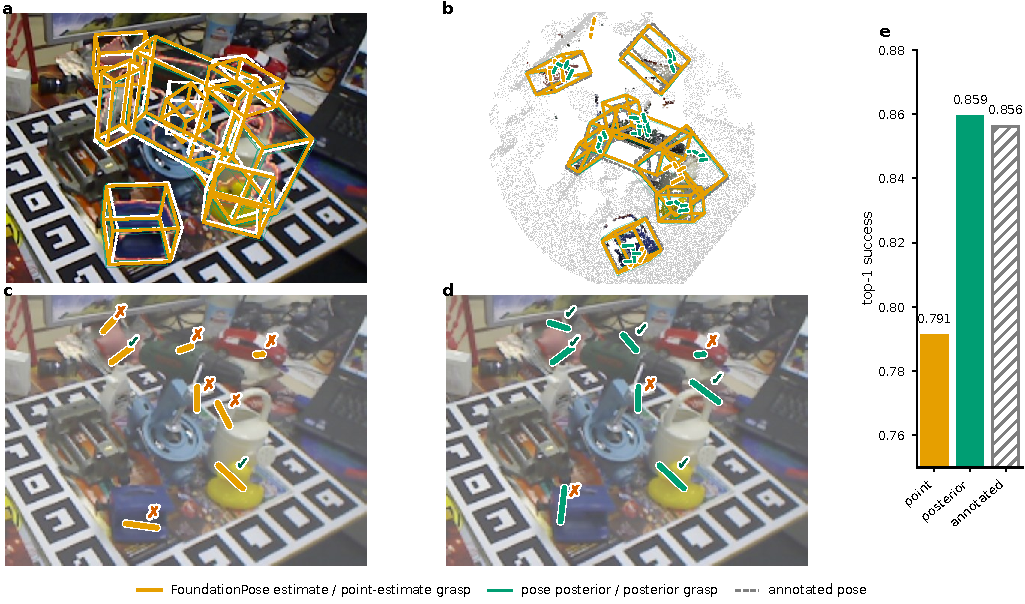
\includegraphics[width=\textwidth]{figures/fig1_teaser.pdf}
\caption{\textbf{Planning on a pose posterior instead of a point estimate.} \textbf{a}, A real LM-O test image with the FoundationPose estimate of every annotated object (orange box), 16 samples of our pose posterior (teal boxes) and the annotated pose (dashed); the heat marks pixels where the posterior samples disagree about the object's extent. \textbf{b}, The same scene as a depth point cloud with the boxes and the grasps chosen by the two planners. \textbf{c}, Grasps chosen on the point estimate (orange) and \textbf{d}, on the posterior (teal); \checkmark\ and $\times$ give the simulated outcome. \textbf{e}, Top-1 grasp success on the \NTest\ LM-Grasp test scenes: point-estimate planning, posterior planning and planning with the annotated pose (hatched). Example frame chosen by a fixed rule (Methods).}\label{fig:teaser}
\end{figure*}

\section{Results}\label{sec:results}

\subsection{Pose-posterior planning}
Fig.~\ref{fig:method} summarises the method. FoundationPose returns a pose $(\hat R,\hat t)$. Observable statistics of how well this pose explains the depth and the mask, together with the viewing direction, locate the frame among the annotated training frames of the same object, and the FoundationPose residuals of its $k=64$ nearest neighbours turn the estimate into pose samples (Methods). Every candidate grasp is simulated at 16 samples under four physics draws and scored by its mean success over these 1,024 rollouts per scene. The robot executes the best candidate, abstains when the conformal certificate fails, or takes a second view when the best score is low.

\begin{figure*}[t]
\centering
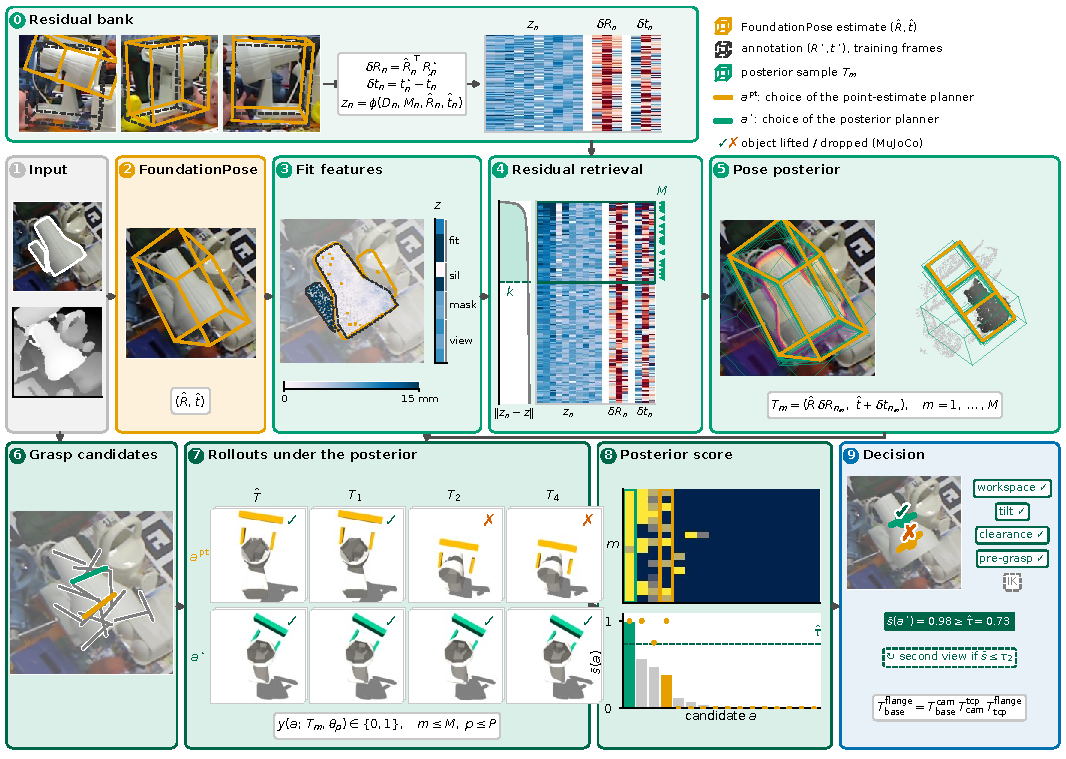
\includegraphics[width=\textwidth]{figures/fig2_method.pdf}
\caption{\textbf{Pose-posterior grasp planning.} (1) A real RGB-D observation with the detection mask. (2) FoundationPose (official weights, frozen) estimates the pose. (3) Observable fit features place the estimate among the annotated training frames of the same object (grey: first two principal components; star: this frame); the residuals of its $k$ nearest neighbours (teal) give pose samples $T_m$, shown as boxes and as the heat of disagreement about the object's extent. (4) Simulated success of every candidate (columns, sorted) under every pose sample, and its posterior mean $\bar s(a)$. (5) The best candidate is executed, rejected, certified, or a second view is requested; the grasp is mapped from the camera to the robot flange. All insets show one real test scene.}\label{fig:method}
\end{figure*}

\subsection{Pose accuracy is a poor proxy for grasp success (RQ1)}
The planner given the annotated pose chooses a successful grasp in \GtTop\ of test scenes, close to the \TestOracle\ of scenes that contain any successful candidate. Perturbing that pose shows how quickly grasps fail while ADD(-S) is still satisfied (Fig.~\ref{fig:posegap}a,b): a rotation error with s.d. $5^\circ$ leaves the ADD(-S) pass rate at \NoiseRotFiveAdd\ and lowers top-1 success to \NoiseRotFiveTop; a translation error of 5\,mm per axis passes on \NoiseTransFiveAdd\ of scenes and lowers success to \NoiseTransFiveTop. FoundationPose operates in this regime (median errors \FpRotErr$^\circ$ and \FpTransErr\,mm). Its planned grasps succeed in \PointTop\ of scenes, \CmpGtPointAbs\ below the annotated pose (95\% CI \CmpGtPointCi), and the loss grows with its error inside the accepted range (Fig.~\ref{fig:posegap}c).

\begin{figure*}[t]
\centering
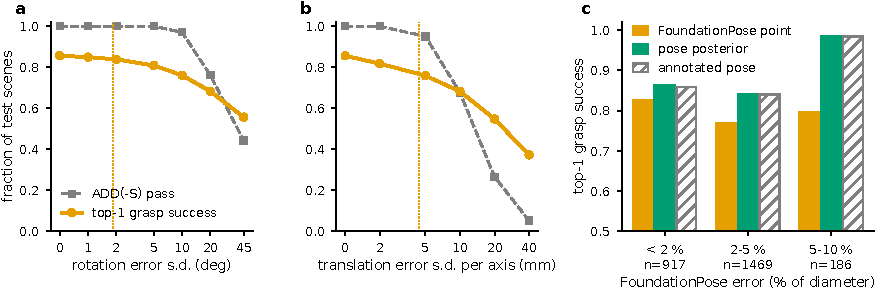
\includegraphics[width=\textwidth]{figures/fig3_pose_gap.pdf}
\caption{\textbf{Pose error versus grasp success on LM-Grasp test scenes.} \textbf{a}, \textbf{b}, The annotated pose perturbed by a random rotation (\textbf{a}) or translation (\textbf{b}) before planning: top-1 grasp success (orange) and the ADD(-S)$<0.1d$ pass rate (dashed); bands: $\pm$ s.d. over three noise seeds; dotted line: median FoundationPose error. \textbf{c}, Top-1 success binned by the FoundationPose ADD(-S) error relative to the object diameter, for planning on the point estimate, on our posterior and on the annotated pose; n: scenes per bin (7 scenes above 10\% not shown).}\label{fig:posegap}
\end{figure*}

\subsection{The posterior recovers annotated-pose grasp success (RQ2)}
Planning on the posterior raises top-1 success from \PointTop\ to \PostTop\ (Table~\ref{tab:main}, Fig.~\ref{fig:results}a), level with the annotated pose (\GtTop; difference \CmpPostGt, 95\% CI \CmpPostGtCi). The gain is largest exactly where the point estimate fails: on the \BinHiN\ scenes with errors between 5\% and 10\% of the diameter, success rises from \BinHiPoint\ to \BinHiPosterior, the annotated-pose value, and on the \BinMidN\ scenes between 2\% and 5\% from \BinMidPoint\ to \BinMidPosterior\ (Fig.~\ref{fig:posegap}c). Of the \NDiffer\ scenes in which the two planners choose different grasps, the posterior's choice succeeds while the point estimate's fails in \NWins, and the reverse happens in \NLosses. A second sampling seed of the posterior gives \PostBTop.

Table~\ref{tab:ablation} rules out two simpler explanations. Monte Carlo averaging alone (the point estimate with the same 1,024 rollouts per scene) reaches \PointSixFourTop, \CmpPostPointSixFourAbs\ below the posterior (CI \CmpPostPointSixFourCi). Generic smoothing (a Gaussian with the residuals' second moments) reaches \GaussTop\ (difference \CmpPostGauss, CI \CmpPostGaussCi) and is poorly calibrated in translation (coverage \CalGaussTransNine\ at 0.9). What matters is the empirical shape of the errors: unconditional resampling of the object's residuals reaches \ObjTop\ (difference \CmpPostObj, CI \CmpPostObjCi), and residuals of the twelve other objects still reach \XoTop, \CmpXoPointSixFourAbs\ above the matched point estimate. The feature conditioning tells the robot which frames are uncertain (rank correlation of predicted spread and realised error \RhoKnnRot\ in rotation and \RhoKnnTrans\ in translation, against \RhoObjRot\ and \RhoObjTrans\ without it; Fig.~\ref{fig:analysis}a,b), although its top-1 gain over unconditional resampling is not significant.

A learned scorer that fuses the image with the planner's score does not add to the posterior planner: the scorer with the posterior score as input (POISE-U) reaches \PoiseUTop, a difference of \CmpPoiseUPost\ to the planner alone (CI \CmpPoiseUPostCi), although the same fusion helps the point-estimate planner (\PoiseTop). Learned outcome scorers without an object model stay well below the FoundationPose-based planners on top-1 success (\EnsTop\ for a deep ensemble).

\begin{table*}[t]
\caption{\textbf{Matched comparison on the LM-Grasp test split} (\NTest\ scenes). n: training seeds (learned methods) or runs; mean $\pm$ s.d. over seeds. Top-1: success of the highest-scoring candidate. AUC: within-scene ranking AUC. Sel@25\%: success on the 25\% of scenes with the most confident choice. Cert.: certified fraction / precision of selection-conditional split conformal prediction at $\alpha=0.1$ (planners without a calibration-split run: --). Shading marks the best and second-best value among non-privileged methods; our rows are tinted. Pose-then-plan methods use the object's mesh, the simulator and the physics prior at decision time.}\label{tab:main}
\centering\footnotesize
\setlength{\tabcolsep}{3.2pt}
\begin{tabular}{lccccc}
\toprule
Method & n & Top-1 & AUC & Sel@25\% & Cert. (fraction / precision)\\
\midrule
\multicolumn{6}{l}{\textcolor{famlearn}{\textbf{Learned outcome scorers (no object model)}}}\\
Dex-Net 2.0 architecture\cite{mahler2017dexnet} & 5 & 0.637 $\pm$ 0.013 & 0.829 & 0.902 & 0.611 / 0.831\\
RGB-D outcome scorer & 5 & 0.683 $\pm$ 0.006 & 0.876 & 0.929 & 0.647 / 0.857\\
Deep ensemble of 5\cite{lakshminarayanan2017} & 3 & 0.705 $\pm$ 0.006 & 0.891 & 0.938 & 0.664 / 0.884\\
\midrule
\multicolumn{6}{l}{\textcolor{famfuse}{\textbf{Learned fusion with the planner score}}}\\
POISE (scorer + point score) & 5 & 0.821 $\pm$ 0.002 & 0.958 & 0.963 & 0.874 / 0.927\\
POISE-U (scorer + posterior score) & 5 & 0.859 $\pm$ 0.002 & \second 0.988 & 0.985 & 0.851 / \second 0.972\\
\midrule
\multicolumn{6}{l}{\textcolor{fampose}{\textbf{Pose-then-plan (mesh, simulator and physics prior at decision time)}}}\\
Pose regressor + planner & 5 & 0.707 $\pm$ 0.007 & 0.859 & 0.817 & --\\
FoundationPose\cite{wen2024foundationpose} + planner & 1 & 0.791 & 0.935 & 0.902 & 0.844 / 0.904\\
FoundationPose + planner, 64 draws & 1 & 0.814 & 0.951 & 0.919 & --\\
\rowcolor{oursrow}\textbf{Pose posterior (ours)} & 1 & \second 0.859 & 0.987 & \second 0.988 & 0.849 / \best 0.972\\
\rowcolor{oursrow}\textbf{+ second view (ours)} & 1 & \best 0.865 & \best 0.993 & \best 0.997 & --\\
\midrule
\multicolumn{6}{l}{\textcolor{famref}{\textbf{Privileged references}}}\\
Annotated pose + planner & 1 & 0.856 & 0.990 & 0.984 & 0.854 / 0.974\\
Oracle (best candidate) & 1 & 0.877 & -- & -- & --\\
\bottomrule
\end{tabular}

\end{table*}

\begin{table*}[t]
\caption{\textbf{What the posterior needs} (LM-Grasp test split). Every row plans the same 16 candidates with common physics draws; rollouts are per scene. Cov@0.9: fraction of scenes whose FoundationPose rotation / translation error lies below the distribution's 90\% quantile (calibrated: 0.90). $\rho$: Spearman correlation between the predicted spread of a frame and its realised error. $\Delta$: paired difference in top-1 success to the point estimate with the same 1,024 rollouts.}\label{tab:ablation}
\centering\footnotesize
\setlength{\tabcolsep}{2.6pt}
\begin{tabular}{lccccccc}
\toprule
 & \multicolumn{2}{c}{Coverage@0.9} & \multicolumn{2}{c}{$\rho$(spread, error)} & & & \\
\cmidrule(lr){2-3}\cmidrule(lr){4-5}
Pose distribution & rot. & trans. & rot. & trans. & Top-1 & $\Delta$ vs 64 draws [95\% CI] & Sel@25\%\\
\midrule
Point estimate, 4 draws & -- & -- & -- & -- & 0.791 & $-$0.023 [$-$0.031, $-$0.016] & 0.902\\
Point estimate, 64 draws & -- & -- & -- & -- & 0.814 & ref. & 0.919\\
Gaussian, matched moments & 0.92 & 0.69 & 0.24 & 0.25 & 0.849 & +0.035 [+0.026, +0.043] & 0.981\\
Bootstrap, unconditional & 0.86 & 0.85 & 0.32 & 0.38 & 0.857 & +0.043 [+0.034, +0.052] & 0.988\\
kNN, other 12 objects & 0.85 & 0.81 & 0.10 & 0.44 & 0.854 & +0.040 [+0.031, +0.049] & 0.981\\
\rowcolor{oursrow}\textbf{kNN, same object (ours)} & 0.87 & 0.84 & 0.40 & 0.65 & 0.859 & +0.045 [+0.036, +0.054] & 0.988\\
\bottomrule
\end{tabular}

\end{table*}

\begin{figure*}[t]
\centering
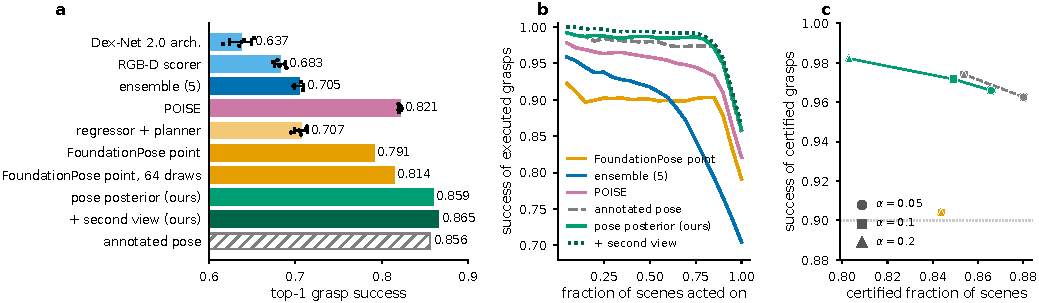
\includegraphics[width=\textwidth]{figures/fig4_results.pdf}
\caption{\textbf{Grasp success and when to act.} \textbf{a}, Top-1 grasp success on the test split; dots: training seeds; error bars: s.d.; light orange: learned pose regressor; hatched: point estimate with the matched rollout budget, and the annotated pose. \textbf{b}, Success of the executed grasps when a method acts only on its most confident fraction of scenes (seed-averaged for learned methods). \textbf{c}, Conformal certificates at $\alpha\in\{0.05,0.1,0.2\}$: fraction of scenes certified and the success of the certified grasps; the point-estimate planner certifies nothing at $\alpha=0.05$.}\label{fig:results}
\end{figure*}

\subsection{Knowing when to act (RQ3)}
The point-estimate planner's score is an average over physics draws at a pose it treats as exact, so it cannot express how reliable that pose is. The posterior score can. On the quarter of scenes where it is most confident, posterior planning succeeds \PostSel\ of the time, against \PointSel\ for the point estimate and \EnsSel\ for the deep ensemble of learned scorers (Fig.~\ref{fig:results}b). Selection-conditional split conformal prediction~\cite{vovk2005,angelopoulos2023} turns the score into a certificate: at $\alpha=0.1$ the posterior planner certifies \PostCertFrac\ of test scenes, and \PostCertPrec\ of the certified grasps succeed, matching the annotated pose (\GtCertPrec) and well above the point estimate (\PointCertPrec\ on \PointCertFrac\ of scenes; Fig.~\ref{fig:results}c). Because a colliding rollout counts as a failure, candidates whose open jaws would hit the object under some of the plausible poses are also ranked down.

\begin{figure*}[t]
\centering
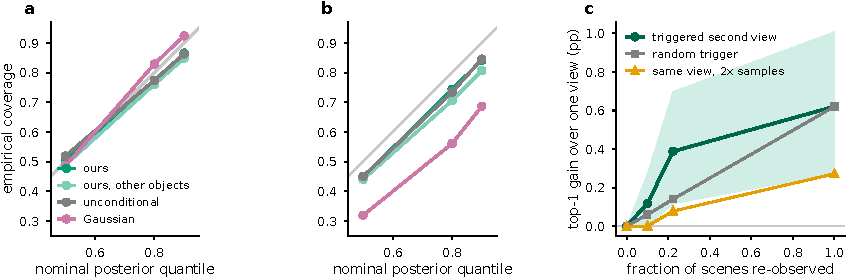
\includegraphics[width=\textwidth]{figures/fig5_analysis.pdf}
\caption{\textbf{Posterior calibration and the value of a second view.} \textbf{a}, \textbf{b}, Fraction of test scenes whose realised FoundationPose rotation (\textbf{a}) and translation (\textbf{b}) error lies below the posterior's 50, 80 and 90\% quantile, for our posterior, the same posterior built from the other twelve objects, unconditional resampling and a moment-matched Gaussian; diagonal: perfect calibration. \textbf{c}, Gain in top-1 success when the least confident scenes are re-observed from a second viewpoint (threshold set on the validation split), against re-observing random scenes and doubling the pose samples of the first view; band: 95\% bootstrap CI of the triggered gain.}\label{fig:analysis}
\end{figure*}

\subsection{A second look and unseen clutter (RQ4)}
LINEMOD sequences show a static scene from a moving camera, so a second view of a scene is another frame of the same sequence, with the camera motion known as it would be from a robot's kinematics. Combining the posteriors of both views helps where the first view is uncertain (Fig.~\ref{fig:analysis}c). With the confidence threshold fixed on the validation split, \SvRate\% of test scenes are re-observed and top-1 success rises by \SvGain\ (95\% CI \SvGainCi), more than by doubling the samples of the first view (difference \SvVsDouble, CI \SvVsDoubleCi); re-observing every scene adds \SvAllGain, so the trigger captures most of the gain for one extra pose estimate (\FpSec\,s) on a fifth of the scenes.

LM-O~\cite{brachmann2014lmo} annotates eight LINEMOD objects in \LmoFrames\ frames of a cluttered sequence with heavy mutual occlusion; no LM-O annotation enters any of our components. With the residual bank, the planner settings and the physics prior unchanged, posterior planning reaches \LmoPostTop\ top-1 success on the \LmoInst\ annotated instances, against \LmoPointTop\ for the point estimate (difference \LmoCmp, 95\% CI \LmoCmpCi) and \LmoGtTop\ with the annotated pose (Fig.~\ref{fig:qualitative}), recovering \LmoRecovered\% of the gap; on its most confident quarter it succeeds \LmoPostSel\ of the time, against \LmoPointSel\ for the point estimate and \LmoGtSel\ with the annotated pose. A gap of \LmoGtMinusPostAbs\ (CI \LmoGtMinusPostCi) remains: occlusion produces larger and differently shaped errors than the LINEMOD frames from which the residual bank is built. The result holds on the instances standing upright on the table (\LmoUpPostTop\ against \LmoUpPointTop; difference \LmoUpCmp, CI \LmoUpCmpCi), where the simulator's upright placement matches the scene exactly.

\begin{figure*}[t]
\centering
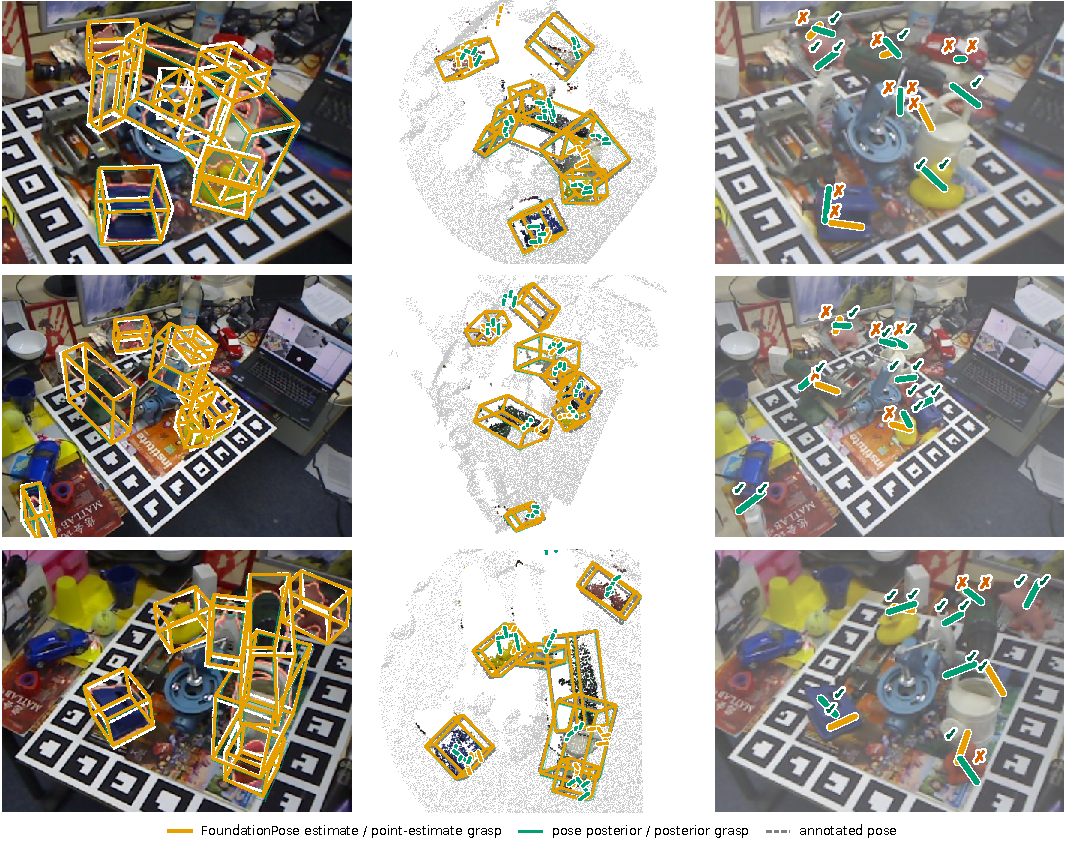
\includegraphics[width=\textwidth]{figures/fig6_qualitative.pdf}
\caption{\textbf{Qualitative results on unseen cluttered LM-O frames.} Each row is one real test image with all annotated objects. Left: FoundationPose estimates (orange boxes), posterior samples (teal boxes) and annotated poses (dashed), with the heat of posterior disagreement. Middle: the depth point cloud with the same boxes. Right: grasps chosen by point-estimate planning (orange) and posterior planning (teal) for every object, with simulated outcomes (\checkmark, $\times$). Frames chosen by a fixed rule (Methods); the last row includes objects on which the posterior's choice fails.}\label{fig:qualitative}
\end{figure*}

\section{Discussion}\label{sec:discussion}
Pose estimators are judged by how close their pose is to the annotation; a grasp planner needs to know how wrong the pose might be. Treating a state-of-the-art estimate as exact cost \CmpGtPointAbs\ in grasp success on real LINEMOD images, and a posterior assembled from the estimator's own residuals recovered all of it, with no change to the estimator, planner or gripper. The mechanism is the classical one of planning under pose uncertainty~\cite{weisz2012poseerror,hsiao2011robust,mahler2016dexnet1}: grasps that survive plausible pose errors are preferred over grasps that succeed only at the estimate. What has been missing for learned render-and-compare estimators is the distribution itself; its empirical shape matters more than a parametric form with the right variance. Because the posterior is built around the estimator, it applies to any estimator whose residuals can be measured on annotated frames, and residuals of other objects are a usable start for an object without annotations.

A trustworthy confidence is the second benefit. The point-estimate planner is most confident exactly when it ignores its pose error, so its certified grasps fail one time in ten; the posterior planner's certified grasps fail as rarely as with the annotated pose. This is what a robot needs to decide whether to act, abstain or look again, and the confidence-triggered second view shows that a single extra observation on the least confident fifth of the scenes buys most of what re-observing every scene would.

Several limitations bound these conclusions. Grasp outcomes are simulated on the scanned meshes, not executed on a robot: the images are real, but friction, mass and centre of mass come from a prior because LINEMOD publishes none, and the planner uses the same simulator and meshes that produced the labels, so all pose-based planners, ours included, face no model mismatch. Every method receives the annotated visible mask, the known-detection assumption of LINEMOD pose studies. The camera motion between views is taken from the annotations, standing in for calibrated arm kinematics. Posterior planning costs 1,024 rollouts per scene (\CpuPost\ CPU-seconds, against \CpuPoint\ for the point estimate), which parallelises across candidates and pose samples but is not yet real-time on embedded hardware. Under the heavy occlusion of LM-O the posterior closes two thirds of the gap rather than all of it, which points to building the residual bank from occluded frames as well. Validating the approach with physical grasps on a robot is the natural next step.

\section{Methods}\label{sec:methods}
\subsection{LM-Grasp}
\paragraph{Images and splits.} We use every real test image of the 13 objects of the standard LINEMOD protocol~\cite{hinterstoisser2012} in the BOP release~\cite{hodan2018bop}, \NScenes\ RGB-D images with one annotated target in clutter. Images are split per object into blocks of 50 consecutive frames assigned to train, validation, calibration or test (probabilities 0.55, 0.10, 0.15, 0.20; \NTrain, \NVal, \NCalib\ and \NTest\ scenes), so near-duplicate frames never straddle two splits. Every method receives the annotated visible mask, the known-detection assumption of LINEMOD pose studies; learned scorers see a $96\times96$ RGB-D crop around it.

\paragraph{Candidates and outcomes.} Each scene receives 16 parallel-jaw candidates built from the observation alone: a visible surface point (with probability 0.7 from the top 5\,cm), an approach tilted by up to $45^\circ$ from the normal of a table plane fitted to the depth image, 0--3\,cm of penetration, at least 4\,cm of table clearance and a random closing angle. Each candidate is mapped into the object frame with the annotated pose and executed in MuJoCo~\cite{todorov2012mujoco} against a CoACD~\cite{wei2022coacd} decomposition of the scanned mesh standing on a table (the model $+z$ axis is within a per-object median of \UprightDegLo--\UprightDegHi$^\circ$ of the fitted table normal). A floating gripper (138\,mm opening, 70\,mm fingers, 10\,N per finger) closes and lifts by 12\,cm; success means the object ends at least 5\,cm above its rest height, and a candidate whose open jaws already intersect the object or the table fails. Friction (log-normal, median 0.5), mass (log-normal around the mesh volume times 500\,kg\,m$^{-3}$) and centre of mass (Gaussian, s.d. 0.15 of the half-extents) are drawn per scene and are invisible to every method; LINEMOD publishes no physical properties, so they are a prior. The corpus holds \NRollouts\ rollouts; on the test split \TestBase\ of candidates succeed and \TestOracle\ of scenes contain a success.

\subsection{Pose estimation}
FoundationPose~\cite{wen2024foundationpose} runs with its official weights on the full RGB-D image, the visible mask, the intrinsics and the mesh, with five refinement iterations (its LINEMOD setting) and the BOP symmetries of eggbox and glue (median \FpSec\,s per image on one NVIDIA RTX PRO 6000).

\subsection{Residual pose posterior}
For a training frame with estimate $(\hat R,\hat t)$ and annotation $(R,t)$ the residual is
\begin{equation}
\delta R=\hat R^{\top}R^{\star},\qquad \delta t=t^{\star}-\hat t,
\end{equation}
where $(R^{\star},t^{\star})$ is the symmetry-equivalent annotation closest in rotation to the estimate. Rotation residuals live in the object frame, where shape ambiguities stay attached to the object; translation residuals live in the camera frame, where depth bias stays along the viewing ray. Ten features are computed from the observation and the estimate only: the median and 90th-percentile distance of up to 3,000 back-projected mask pixels to the posed mesh surface, the fraction farther than 10\,mm, the fraction of the projected model silhouette covered by the mask, the fraction of the mask outside it, the valid-depth fraction, the log mask area, and the camera direction in the estimated object frame. For a frame of object $o$, features are standardised by the per-object median and interquartile range of the bank (all \NTrain\ training frames), and $M=16$ residuals are drawn without replacement from the $k=64$ nearest bank frames of $o$, a nearest-neighbour residual bootstrap~\cite{efron1979bootstrap,lall1996nnboot}; pose samples are $T_m=(\hat R\,\delta R_m,\ \hat t+\delta t_m)$. Bank frames of the same object within one 50-frame block of the query are excluded in every split, so no frame draws its own residual or a near-duplicate's. Controls with the same budget: a Gaussian with each object's root-mean-square residual angle about a random axis and per-axis translation s.d.; unconditional resampling of the object's residuals; and the $k$ nearest frames of the other twelve objects on the seven object-agnostic features.

\subsection{Planning under the posterior}
A candidate $a$ is simulated with the object at every sample $T_m$ under $P=4$ physics draws $\theta_p$ (the nominal parameters and three prior samples, common to all candidates and samples) and scored by
\begin{equation}
\bar s(a)=\frac{1}{MP}\sum_{m=1}^{M}\sum_{p=1}^{P} y\big(a;\,T_m,\theta_p\big),
\end{equation}
where $y\in\{0,1\}$ is the simulated success and a colliding rollout counts as a failure. The evaluated planner selects the highest $\bar s$; the point-estimate planner is the case $M=1$ at $(\hat R,\hat t)$, the annotated-pose planner uses $(R,t)$. For execution, the selected grasp is mapped as $T^{\mathrm{flange}}_{\mathrm{base}}=T^{\mathrm{cam}}_{\mathrm{base}}T^{\mathrm{tcp}}_{\mathrm{cam}}T^{\mathrm{flange}}_{\mathrm{tcp}}$ and checked against the workspace, approach tilt, table clearance and the arm's inverse kinematics; the interface reports the reason for every rejection (collision, low $\bar s$, failed certificate or kinematic check). No physical motion was executed in this study.

\subsection{Second view}
The second view of a test frame is the frame of its 50-frame block whose viewing direction differs most from the current one, up to $30^\circ$ (median \SvViewDeg$^\circ$). Its estimate and posterior samples are mapped into the current camera with the camera motion $T_{c_i c_j}=T_{c_i o}T_{c_j o}^{-1}$ of the static scene, computed from the annotations as a stand-in for arm kinematics, and the planner uses the 32 samples of both views. A scene is re-observed when $\bar s$ of its selected grasp is at most a threshold fixed on the validation split at a 25\% rate.

\subsection{Learned baselines and fusion}
The learned scorers share an ImageNet-initialised ResNet-18~\cite{he2016resnet,deng2009imagenet} with an RGB-D stem and an outcome head in which a 32-dimensional image code modulates each candidate's action embedding; the deep ensemble~\cite{lakshminarayanan2017} averages five seeds. The Dex-Net 2.0 grasp-quality architecture~\cite{mahler2017dexnet} scores a depth patch aligned with each candidate. A pose regressor (six-dimensional rotation~\cite{zhou2019rotation} and translation) feeds the planner. POISE and POISE-U append the point-estimate or posterior planner score to each candidate's features. All are trained on the same data for 20 epochs with AdamW~\cite{loshchilov2019adamw} (Adam for the Dex-Net architecture), identical augmentation and checkpoint selection on validation loss, with five seeds.

\subsection{Selection protocol}
Every design choice (posterior features, $k$, residual frames, controls, second-view rule, fusion variants) was fixed in a written plan before it was run and selected on the validation split; the posterior planner, its controls and the fusion variants were then evaluated on the test split once, in a single pass (baseline test results had been computed earlier and were not revisited). The LM-O protocol, including the visibility cut and the upright subset, was fixed before any LM-O result was computed. Example frames in Figs.~\ref{fig:teaser} and \ref{fig:qualitative} are the LM-O frames in which the posterior's choice succeeds and the point estimate's fails for the most objects, plus the frame with the most objects where the reverse holds.

\subsection{LM-O transfer check}
We use the 200 BOP test frames of LM-O~\cite{brachmann2014lmo} and every annotated instance with visible fraction at least 0.1. Observations, candidates, physics prior, simulator and FoundationPose settings follow LM-Grasp, with outcomes simulated at the LM-O annotation, and the residual bank is the LM-Grasp training split. Because the simulator stands objects upright, we also report the instances whose model $+z$ axis is within $15^\circ$ of the fitted table normal (\LmoUpright\ of instances).

\subsection{Metrics and statistics}
\emph{Top-1 success} is the outcome of the highest-scoring candidate averaged over scenes (ties broken by a fixed jitter shared by all methods). \emph{Within-scene AUC} is the ROC area among a scene's candidates, averaged over the \NMixed\ test scenes with both outcomes. \emph{Selective success} at coverage $c$ is the top-1 success on the fraction $c$ of scenes with the highest score of the selected candidate. The \emph{certificate} is selection-conditional split conformal prediction~\cite{vovk2005,angelopoulos2023} calibrated on the selected candidate of each calibration scene (nonconformity $1-\hat p$ for successes, $\hat p$ for failures); a scene is certified when the prediction set of its selected candidate is $\{\text{success}\}$. Pose accuracy is the ADD (ADD-S for eggbox and glue~\cite{hodan2016eval}) pass rate at 10\% of the diameter. Posterior calibration is the fraction of scenes whose realised error lies below a quantile of the posterior samples' errors. Differences in top-1 success are paired bootstraps over scenes (10,000 resamples), seed-averaged for learned methods, reported with 95\% percentile intervals; learned methods report mean $\pm$ s.d. over seeds. Software: Python 3.12, PyTorch 2.14, MuJoCo 3.10; FoundationPose in its own environment (PyTorch 2.7.1, CUDA 12.8); two-view planning costs \CpuTwoView\ CPU-seconds per scene.

\subsection{Use of large language models}
Claude (Anthropic) was used to write and run experiment code and to draft the manuscript text under the authors' direction. All reported numbers are produced by the released scripts from the stored results files.


\backmatter

\bmhead{Data availability}
LINEMOD and LM-O are available from the BOP benchmark (\url{https://bop.felk.cvut.cz}). The LM-Grasp corpus is generated deterministically from LINEMOD by the released scripts; the generated corpus, pose estimates, posterior samples and all results files are available from the corresponding author on reasonable request.

\bmhead{Code availability}
The code that builds LM-Grasp, computes the pose posteriors, plans and evaluates every method and regenerates every figure, table and number in this article will be released at \url{https://github.com/s-elim/msp-framework} upon publication.

\bmhead{Acknowledgements}
[To be completed by the authors.]

\bmhead{Author contributions}
M.S.S. conceived the study, developed the method and the benchmark, ran the experiments and wrote the manuscript. S.K. supervised the work and revised the manuscript. [To be confirmed by the authors.]

\bmhead{Competing interests}
The authors declare no competing interests.

\bibliography{refs}

\end{document}
